% =====================================================================
% Rozdział 5 – Implementacja (WZÓR, ok. 6 stron)
% Styl bezosobowy. Klucze \cite{} – literatura_wzor.bib (klucze z bibliografii autora).
% Rysunki: rysunki/rejestracja_para14.pdf, rysunki/panderm_trening.png.
% Wymaga pakietów: booktabs, tabularx, amsmath, algorithm, algpseudocode (opcja noend) – polskie
% nazwy w preambule (wzor_podglad.tex). Plan i zwroty: materialy/06_plan_zwroty_rozdzialy_4_7.md.
% Przy braku miejsca: usuń rys. fig:panderm-trening (wynik testu ISIC zostaje w tekście).
% =====================================================================

\chapter{Implementacja}
\label{chap:implementacja}

W rozdziale opisano implementację modułów systemu: przygotowanie danych, rejestrację, modele segmentacji, przeniesienie obszarów wraz z zapisem pikseli znamienia, pomiary oraz bazę danych, raport i aplikację. System zaimplementowano w języku Python; instalację środowisk i strukturę kodu opisano w dokumentacji technicznej (Dodatek~B).

\section{Akwizycja i przygotowanie danych}
\label{sec:dane}

Zbiór danych zebrano w jednej serii pomiarowej 23 października 2026~r. Obejmuje on 94 pary obrazów przedstawiających 34 znamiona; każde znamię sfotografowano dwa lub trzy razy, zmieniając obrót znacznika, odległość i kąt wykonania zdjęcia. Zdjęcia wykonano telefonem w formacie HEIC i przekonwertowano do formatu JPG (dłuższy bok 1104--3274 pikseli). Obrazy termowizyjne zarejestrowano kamerą FLIR A320 z obiektywem 18~mm jako nagrania .SEQ o rozdzielczości 320~$\times$~240 pikseli. Z pierwszej klatki każdego nagrania wyznaczono:
\begin{itemize}
  \item obraz podglądowy z paletą barw, znormalizowany do zakresu między 2. a 98. percentylem wartości nagrania -- wykorzystywany w rejestracji i wizualizacji;
  \item macierz surowych wartości detektora (liczby całkowite 16-bitowe), wykorzystywaną jako intensywność pikseli znamienia (WF15);
  \item pomocniczo -- mapę temperatur obliczoną z parametrów zapisanych w nagraniu przy emisyjności skóry 0,98~\cite{infared-thermal-imaging}.
\end{itemize}
Przy odczycie usuwano dolne wiersze zawierające dane telemetryczne kamery. Zgodność pikseli wszystkich reprezentacji sprawdzono współczynnikiem korelacji rang, który dla każdej z 94 par wyniósł co najmniej 0,95.

Ręczne adnotacje wykonano w programie CVAT: maskę znamienia na zdjęciu, maski znacznika na obu obrazach oraz osiem narożników znacznika w każdej modalności. Z narożników wyznaczono homografię przekształcającą piksele na milimetry w płaszczyźnie znacznika. Adnotacje wykorzystano wyłącznie do oceny wyników oraz do uczenia modelu M3. Na potrzeby walidacji krzyżowej zbiór podzielono na pięć foldów według znamion, a nie zdjęć, aby zdjęcia tego samego znamienia nie trafiały jednocześnie do zbioru uczącego i testowego.

\section{Moduł rejestracji}
\label{sec:impl-rejestracja}

Rejestrację zrealizowano zgodnie z założeniem przyjętym w rozdziale~\ref{chap:projekt}: transformację wyznacza się na podstawie znacznika $\Pi$, a nie całej sceny. Przebieg metody przedstawiono w postaci pseudokodu (algorytm~\ref{alg:rejestracja}), a jej wynik dla przykładowej pary -- na rysunku~\ref{fig:rejestracja-para}.

\subsection{Detekcja znacznika}

Na obrazie termowizyjnym folia odbija promieniowanie otoczenia, dlatego jest ciemniejsza od skóry albo -- przy odbiciach obiektów o różnej temperaturze -- silnie teksturowana, podczas gdy skóra jest gładka. Kandydatów na znacznik wyznaczono jako spójne obszary ciemniejsze od skóry (progi 0,5, 0,65 i 0,8 wartości 70. percentyla jasności obrazu) lub o lokalnym odchyleniu standardowym jasności większym niż 6, 10 albo 15, po otwarciu i zamknięciu morfologicznym. Spośród kandydatów wybierano obszar najbardziej podobny do wzorca $\Pi$; miarą podobieństwa jest indeks Jaccarda (IoU) kandydata i wzorca o tym samym polu i środku masy, maksymalizowany względem kąta obrotu w zakresie 0--360° z krokiem 4°. Krawędź folii, rozmytą przez optykę kamery, wyznaczono z dokładnością subpikselową, przyjmując w pasie $\pm 4$~pikseli wokół krawędzi próg w połowie między jasnością folii i skóry.

Na zdjęciu folia jest chłodniejsza w barwie od skóry -- ma mniejszą sumę składowych $a^*$ i $b^*$ przestrzeni L*a*b* niż mediana skóry -- i ma teksturę załamań. Kandydatów wyznaczono przy kilku progach z mapy barwy, mapy tekstury (odchylenie standardowe w oknie 7~$\times$~7 pikseli) oraz ich połączenia, a wybór przebiega tak samo jak na obrazie termowizyjnym. Krawędź folii doprecyzowano segmentacją interaktywną z biblioteki OpenCV, akceptowaną tylko wtedy, gdy nie pogarsza zgodności kształtu z wzorcem. Detekcję na zdjęciu wykonuje się w skali roboczej, w której dłuższy bok ma 1000 pikseli. Jeżeli zgodność wykrytego obiektu z wzorcem jest mniejsza niż 0,65, system zgłasza ostrzeżenie (WN6).

\subsection{Dopasowanie wstępne i doprecyzowanie metodą ECC}

Dopasowanie wstępne jest przekształceniem przez podobieństwo: przesunięcie wynika ze środków mas masek znacznika, skala -- z pierwiastka stosunku ich pól, a kąt -- z maksimum IoU masek po obrocie (krok 2°, a następnie $\pm 2^\circ$ z krokiem 0,25°). Transformację doprecyzowano, maksymalizując kryterium ECC~\cite{evangelidis2008} funkcją \texttt{findTransformECC} biblioteki OpenCV. Kryterium obliczano nie na intensywnościach obrazów, lecz na maskach znacznika rozmytych filtrem Gaussa, co sprowadza problem wielomodalny do jednomodalnego (podrozdział~\ref{sec:modele-transformacji}). Optymalizację prowadzono od dużego do małego rozmycia: dla przekształcenia afinicznego przy $\sigma = 6$, 3 i 1,5~piksela, a następnie dla homografii przy $\sigma = 3$ i 1,5~piksela (do 200 iteracji, $\varepsilon = 10^{-6}$), na wycinku obejmującym znacznik z marginesem 30\%. Rozmycie poszerza obszar zbieżności metody gradientowej, a jego stopniowe zmniejszanie zwiększa dokładność.

\subsection{Wybór modelu przekształcenia}

Domyślnie przyjmowano przekształcenie afiniczne. Homografię wybierano wtedy, gdy zmniejszała średni błąd krawędzi masek o ponad 5\% i była stabilna, tzn. lokalna skala pola w narożnikach kadru zdjęcia różniła się od skali w środku znacznika najwyżej dwukrotnie. Warunek ten odrzuca homografie dopasowane do znacznika, ale zniekształcające pozostałą część obrazu. W zbiorze 92 przeanalizowanych par homografię wybrano 65 razy, a przekształcenie afiniczne -- 27 razy. Wynikiem modułu jest macierz $T$ przekształcająca piksel zdjęcia na piksel obrazu termowizyjnego, obraz termowizyjny w geometrii zdjęcia (z kanałem przezroczystości wyznaczającym pole widzenia kamery) oraz nałożenie obu obrazów.

\begin{algorithm}[htbp]
  \caption{Rejestracja zdjęcia i obrazu termowizyjnego na podstawie znacznika $\Pi$}
  \label{alg:rejestracja}
  \small
  \begin{algorithmic}[1]
    \Require zdjęcie $I_R$, obraz termowizyjny $I_T$, wzorzec $\Pi$
    \Ensure macierz $T$ (piksel $I_R$ $\to$ piksel $I_T$), model przekształcenia
    \State $M_T \gets$ \Call{WykryjZnacznik}{$I_T$} \Comment{obszary ciemne lub teksturowane}
    \State $M_R \gets$ \Call{WykryjZnacznik}{$I_R$} \Comment{obszary chłodne w barwie lub teksturowane}
    \If{$\mathrm{IoU}(M_R, \Pi) < 0{,}65$ \textbf{lub} $\mathrm{IoU}(M_T, \Pi) < 0{,}65$}
      \State zgłoś ostrzeżenie o niepewnej detekcji znacznika
    \EndIf
    \State $W_0 \gets$ podobieństwo: środki mas, skala $\sqrt{|M_T| / |M_R|}$, kąt $\arg\max_\alpha \mathrm{IoU}\big(\mathrm{obrót}_\alpha(M_R), M_T\big)$
    \State $W_A \gets W_0$
    \For{$\sigma \in (6;\ 3;\ 1{,}5)$}
      \State $W_A \gets \mathrm{ECC}_{\mathrm{afiniczne}}(G_\sigma * M_R,\ G_\sigma * M_T,\ W_A)$
    \EndFor
    \State $W_H \gets W_A$
    \For{$\sigma \in (3;\ 1{,}5)$}
      \State $W_H \gets \mathrm{ECC}_{\mathrm{homografia}}(G_\sigma * M_R,\ G_\sigma * M_T,\ W_H)$
    \EndFor
    \If{$e(W_H) < 0{,}95\, e(W_A)$ \textbf{oraz} $W_H$ stabilna} \Comment{$e$ -- średni błąd krawędzi masek}
      \State \Return $W_H$, homografia
    \Else
      \State \Return $W_A$, przekształcenie afiniczne
    \EndIf
  \end{algorithmic}
\end{algorithm}

\begin{figure}[htbp]
  \centering
  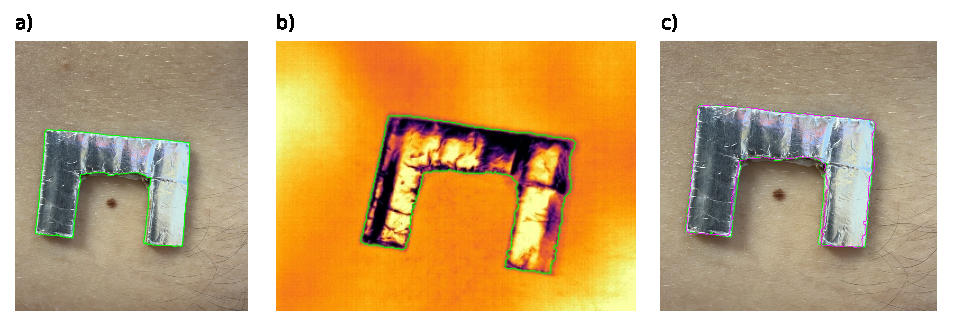
\includegraphics[width=0.92\textwidth]{rysunki/rejestracja_para14.pdf}
  \caption{Rejestracja pary 14: a)~folia wykryta na zdjęciu, b)~folia wykryta na obrazie termowizyjnym, c)~kontur folii ze zdjęcia (zielony) i kontur folii z obrazu termowizyjnego przeniesiony przekształceniem odwrotnym do $T$ (fioletowy). Źródło: opracowanie własne}
  \label{fig:rejestracja-para}
\end{figure}

\section{Modele segmentacji}
\label{sec:impl-segmentacja}

Zgodnie z celem pracy każda modalność ma własny model segmentacji. Na zdjęciu segmentowane jest znamię (model M1), a na obrazie termowizyjnym -- znacznik (model M3), ponieważ znamię nie jest na nim widoczne. Parametry uczenia obu modeli zestawiono w tabeli~\ref{tab:uczenie}.

\begin{table}[htbp]
  \centering
  \caption{Parametry uczenia modeli segmentacji}
  \label{tab:uczenie}
  \small
  \begin{tabularx}{\textwidth}{>{\raggedright\arraybackslash}p{2.6cm} >{\raggedright\arraybackslash}X >{\raggedright\arraybackslash}X}
    \toprule
    Parametr & M1: PanDerm + UperNet & M3: U-Net \\
    \midrule
    zadanie & znamię na zdjęciu & znacznik na obrazie termowizyjnym \\
    dane uczące & ISIC 2018 Task 1: 2594 / 100 / 1000 obrazów & 94 obrazy własne, 5 foldów według znamion \\
    wejście & 224~$\times$~224, RGB & 240~$\times$~320, skala szarości \\
    architektura & koder ViT-L z wagami PanDerm, dekoder UperNet & U-Net, kanały 16--256, 1,94~mln parametrów \\
    funkcja straty & entropia krzyżowa & BCE + (1 $-$ miękki Dice) \\
    optymalizator & AdamW (8-bitowy), $\eta = 10^{-4}$, $\lambda = 0{,}05$ & AdamW, $\eta = 2\cdot10^{-3}$, $\lambda = 10^{-4}$ \\
    harmonogram & kosinusowy, 100 epok, wybór epoki na zbiorze walidacyjnym & kosinusowy, 60 epok, bez wyboru epoki \\
    paczka & 2 & 8 \\
    augmentacja & zmiany barw, skala szarości, autokontrast, negatyw & obrót 0--360°, skala 0,75--1,3, przesunięcie, odbicia, korekcja gamma, kontrast, rozmycie, szum \\
    uruchamianie & PyTorch, osobny proces & ONNX + OpenCV w aplikacji \\
    \bottomrule
  \end{tabularx}
\end{table}

\subsection{Model M1 -- znamię na zdjęciu}

Model M1 składa się z kodera PanDerm (transformer wizyjny ViT-L) z wagami udostępnionymi przez autorów~\cite{yan2025panderm} oraz dekodera UperNet~\cite{xiao2018upernet}. Model douczono na zbiorze ISIC 2018 Task~1~\cite{codella2019} według procedury autorów modelu PanDerm; ze względu na kartę graficzną o pamięci 8~GB zastosowano 8-bitową wersję optymalizatora AdamW i obliczenia w formacie bfloat16. Model wybrano po 11. epoce, w której indeks Jaccarda na zbiorze walidacyjnym był największy (rys.~\ref{fig:panderm-trening}). Na zbiorze testowym (1000 obrazów) uzyskano współczynnik Dice'a 0,899 i indeks Jaccarda 0,833.

% OPCJA (ok. 0,4 s.): przy braku miejsca usuń rysunek i odwołanie do niego -- wynik testu ISIC zostaje w tekście.
\begin{figure}[htbp]
  \centering
  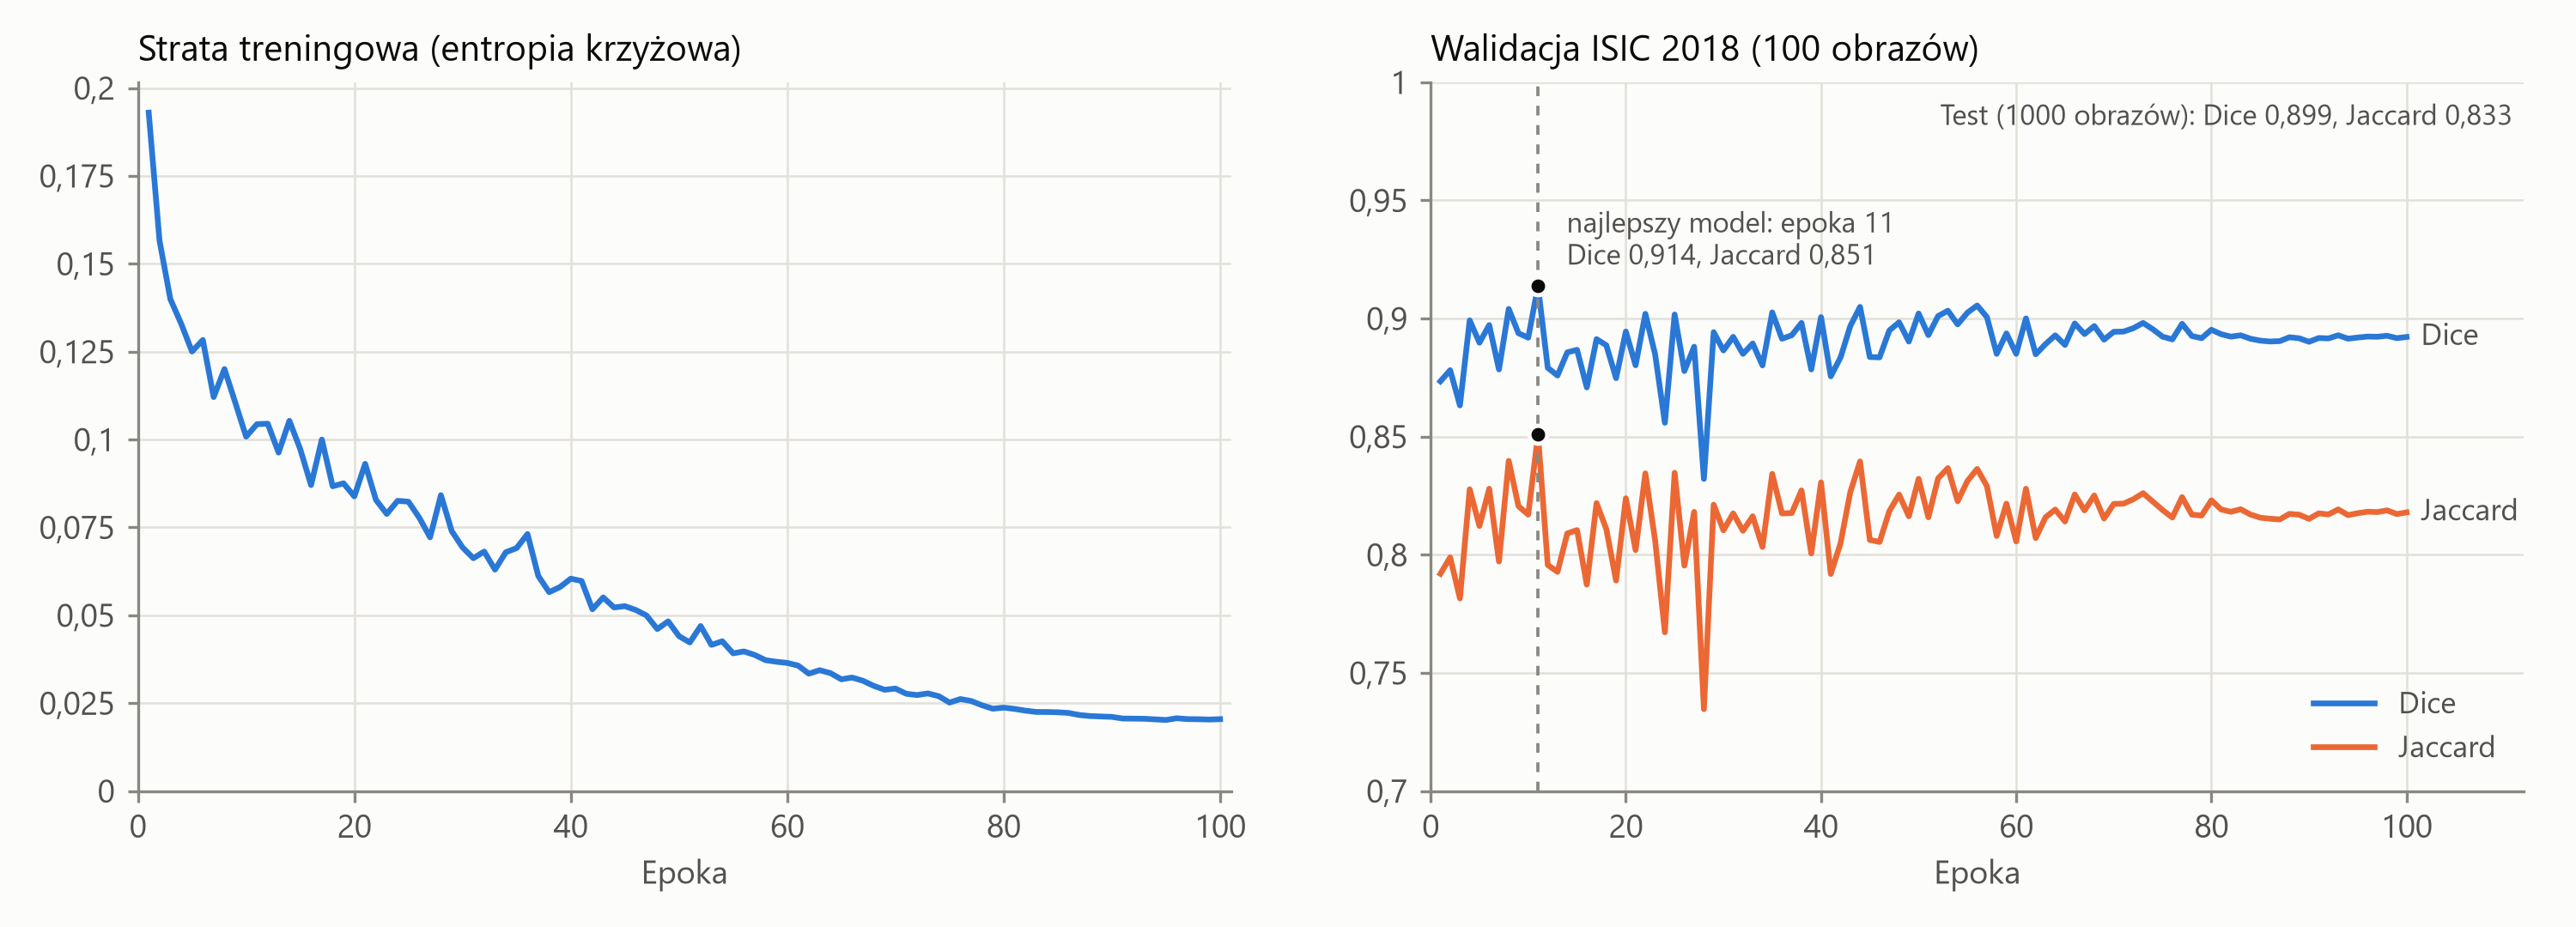
\includegraphics[width=0.85\textwidth]{rysunki/panderm_trening.png}
  \caption{Douczanie modelu M1 na zbiorze ISIC 2018: strata na zbiorze uczącym (po lewej) oraz współczynnik Dice'a i indeks Jaccarda na zbiorze walidacyjnym (po prawej). Źródło: opracowanie własne}
  \label{fig:panderm-trening}
\end{figure}

Bezpośrednie zastosowanie modelu do zdjęć z telefonu dawało maski znacznie zawyżone. Przyczyną jest przesunięcie dziedziny: w obrazach dermatoskopowych ISIC znamię zajmuje około połowy kadru, a na zdjęciu ze znacznikiem znamię o średnicy 1--4~mm zajmuje niewielką część otworu o boku 17~mm. Dlatego obszar segmentacji ograniczono do otworu znacznika poszerzonego o 8\% (piksele folii zastępuje się medianą barwy skóry), a segmentację podzielono na dwa kroki. Najpierw wyznacza się do trzech kandydatów na znamię jako plamy ciemniejsze od lokalnego tła skóry: jasność po domknięciu morfologicznym o promieniu ok. 0,2~mm, usuwającym włosy, porównuje się z medianą w oknie 8~mm, odrzucając pasy wzdłuż folii i kształty wydłużone. Następnie model segmentuje kadr wokół każdego kandydata, dobrany tak jak w danych uczących ISIC (znamię zajmuje ok. 53\% dłuższego boku kadru), a spośród wyników wybiera się maskę o największym kontraście brzegu, czyli różnicy jasności wewnątrz maski i w pasie 0,4~mm na zewnątrz niej. Model M1 działa w osobnym środowisku z biblioteką PyTorch i jest uruchamiany przez aplikację jako odrębny proces (WN7).

\subsection{Model M3 -- znacznik na obrazie termowizyjnym}

Model M3 jest siecią U-Net~\cite{ronneberger2015} zmniejszoną do rozmiaru zbioru: koder i dekoder mają cztery poziomy o liczbie kanałów 16, 32, 64 i 128, a najgłębsza warstwa -- 256 kanałów. Każdy z dziewięciu bloków składa się z dwóch splotów 3~$\times$~3 z normalizacją wsadową i funkcją aktywacji ReLU; sieć ma 1,94~mln parametrów. Wejściem jest obraz termowizyjny w skali szarości, standaryzowany osobno dla każdego obrazu, a wyjściem -- mapa prawdopodobieństwa przynależności piksela do folii, progowana wartością 0,5. Sieć uczono na 94 maskach znacznika z programu CVAT w 5-krotnej walidacji krzyżowej według znamion; dla każdej pary system używa modelu foldu, w którym była ona w zbiorze testowym, a dla obrazów spoza zbioru -- modelu uczonego na wszystkich parach. Liczbę epok ustalono z góry, bez wyboru epoki na zbiorze testowym, aby nie zawyżać wyników, a niewielki rozmiar zbioru kompensowano silną augmentacją. Wytrenowane sieci wyeksportowano do formatu ONNX i uruchamia się je modułem \texttt{dnn} biblioteki OpenCV, bez biblioteki PyTorch; segmentacja jednego obrazu trwa ok.~67~ms na procesorze (WN2). Model M3 nie uczestniczy w rejestracji, dlatego jego maska stanowi niezależny punkt odniesienia w badaniu E2.

\section{Przeniesienie obszarów i skala metryczna}
\label{sec:impl-przeniesienie}

Skalę metryczną wyznaczono z narożników znacznika. Wzorzec $\Pi$ o znanych wymiarach dopasowano do maski znacznika w każdej modalności (podobieństwo, a następnie ECC dla przekształcenia afinicznego i homografii), a osiem wierzchołków dopasowanego wzorca przyjęto za narożniki. Z narożników wyznaczono homografię $H$ przekształcającą piksele obrazu na milimetry w płaszczyźnie znacznika. Lokalny rozmiar piksela w danym punkcie jest pierwiastkiem z wartości bezwzględnej wyznacznika jakobianu $H$; dla obrazu termowizyjnego wynosi on 0,21--0,44~mm (mediana 0,28~mm).

Obszary przenoszono wektorowo (algorytm~\ref{alg:przeniesienie}). Kontur maski znamienia na zdjęciu, poszerzony o pół piksela (kontur prowadzony przez środki pikseli brzegowych zaniżałby pole), przekształcano macierzą $T$, a powstały wielokąt wypełniano w siatce czterokrotnie gęstszej niż piksele obrazu termowizyjnego. Średnia w bloku 4~$\times$~4 daje ułamek pokrycia każdego piksela przez znamię (wielokrotność 1/16). Pozwala to zachować kształt małego obszaru -- znamię obejmuje na obrazie termowizyjnym od 10 do 290 pikseli -- przy błędzie pola rzędu 1\%. W ten sam sposób przenoszono obrys i otwór znacznika.

Dla każdego piksela obrazu termowizyjnego o niezerowym ułamku pokrycia system zapisuje jego współrzędne $x$ (kolumna) i $y$ (wiersz), ułamek pokrycia oraz surową intensywność odczytaną z nagrania .SEQ (WF15). Piksel uznaje się za należący do znamienia, gdy znamię pokrywa co najmniej połowę jego pola, co odpowiada przeniesieniu maski binarnej. Pozostałe piksele są zapisywane wraz z ułamkiem pokrycia, co umożliwia analizę z wagami. Lista pikseli trafia do pliku CSV i do tabeli \texttt{piksel} bazy danych.

\begin{algorithm}[htbp]
  \caption{Przeniesienie znamienia na obraz termowizyjny i zapis pikseli}
  \label{alg:przeniesienie}
  \small
  \begin{algorithmic}[1]
    \Require maska znamienia $Z$ na zdjęciu, macierz $T$, surowe wartości detektora $I$ ($320 \times 240$)
    \Ensure lista pikseli $(x, y, u, m, I(x, y))$
    \State $K \gets$ kontur maski $Z$ poszerzony o pół piksela
    \State $K' \gets T \cdot K$ \Comment{wierzchołki we współrzędnych obrazu termowizyjnego}
    \State $G \gets$ wypełnienie wielokąta $K'$ w siatce $1280 \times 960$ \Comment{4 razy gęstszej}
    \ForAll{piksele $(x, y)$ obrazu termowizyjnego}
      \State $u \gets$ średnia $G$ w bloku $4 \times 4$ odpowiadającym pikselowi $(x, y)$
      \If{$u > 0$}
        \State $m \gets [\,u \geq 0{,}5\,]$ \Comment{piksel w masce znamienia}
        \State dopisz $(x, y, u, m, I(x, y))$ do listy
      \EndIf
    \EndFor
    \State zapisz listę do pliku CSV i tabeli \texttt{piksel}
  \end{algorithmic}
\end{algorithm}

\section{Pomiary i miary zgodności}
\label{sec:impl-pomiary}

Parametry znamienia oblicza się na zdjęciu, przeliczając kontur maski na milimetry homografią $H$. Wyznaczane są: pole $P$, obwód $L$, średnica równoważna $d = 2\sqrt{P/\pi}$, maksymalna i minimalna średnica Fereta (z otoczki wypukłej i najmniejszego prostokąta opisanego), kolistość $4\pi P / L^2$, asymetria względem osi głównej i osi prostopadłej -- jako część pola niepokryta po odbiciu kształtu względem danej osi -- oraz średnia barwa w przestrzeni L*a*b* (WF8).

Miary zgodności dwóch masek $A$ i $B$ (podrozdział~\ref{sec:miary}) oblicza się w siatce czterokrotnie gęstszej niż piksele obrazu termowizyjnego, aby schodkowy brzeg pikseli nie zaniżał wyniku. Są to: współczynnik Dice'a, indeks Jaccarda (IoU), stosunek pól $|A|/|B|$, przesunięcie środków ciężkości oraz HD95 i ASSD obliczane z transformaty odległości brzegów masek; odległości przelicza się na milimetry lokalnym rozmiarem piksela. Błąd TRE~\cite{fitzpatrick1998} jest średnią odległością ośmiu narożników znacznika oznaczonych na zdjęciu i przeniesionych macierzą $T$ od narożników oznaczonych na obrazie termowizyjnym, mierzoną w milimetrach w płaszczyźnie znacznika:
\begin{equation}
  \mathrm{TRE} = \frac{1}{8}\sum_{i=1}^{8} \left\| H_T\!\left(T\,p_i^{R}\right) - H_T\!\left(p_i^{T}\right) \right\|,
  \label{eq:tre}
\end{equation}
gdzie $p_i^{R}$ i $p_i^{T}$ to $i$-ty narożnik na zdjęciu i na obrazie termowizyjnym, a $H_T$ -- homografia obrazu termowizyjnego (piksele $\to$ mm).

W badaniu E2 maską $A$ jest folia znacznika wykryta na zdjęciu przez detektor modułu rejestracji i przeniesiona macierzą $T$, a maską $B$ -- folia wyznaczona na obrazie termowizyjnym przez model M3. Otwór znacznika, czyli obszar zainteresowania, wyznacza się dla obu masek tą samą funkcją -- jako otoczkę wypukłą maski pomniejszoną o folię.

\section{Baza danych, raport i aplikacja}
\label{sec:impl-aplikacja}

Bazę danych zaimplementowano z użyciem modułu \texttt{sqlite3} biblioteki standardowej języka Python. Schemat jest zdefiniowany w kodzie i ma numer wersji; baza tworzy się automatycznie przy pierwszym zapisie analizy, a przy otwarciu bazy w starszej wersji dopisywane są brakujące tabele. Po każdej analizie zapisywany jest wiersz w tabeli \texttt{analiza}, wszystkie wartości liczbowe wyników w tabeli \texttt{miara} oraz piksele znamienia w tabeli \texttt{piksel}; nieudana analiza jest zapisywana ze statusem błędu i jego opisem. Obsługę bazy z wiersza poleceń -- import danych, podsumowanie, eksport wyników i pikseli do plików CSV oraz dowolne zapytania SQL -- zapewnia skrypt \texttt{baza\_danych.bat}.

Raport pary jest pojedynczym plikiem HTML z osadzonymi obrazami, który można otworzyć w dowolnej przeglądarce. Zawiera opis wykonanych etapów, obrazy (znacznik i narożniki, nałożenie, powiększenie wokół znamienia, maski badania E2, piksele znamienia), tabele wyników i objaśnienie każdej wielkości. System dodaje uwagi, gdy wynik wymaga sprawdzenia, np. gdy błąd TRE przekracza 1~mm, współczynnik Dice'a w badaniu E2 jest mniejszy niż 0,85, zgodność znacznika z wzorcem jest mniejsza niż 0,65 lub brakuje nagrania .SEQ. Obok raportu zapisywane są plik \texttt{metryki.json} z wynikami liczbowymi, obrazy PNG i plik CSV z pikselami znamienia.

Aplikację okienkową zaimplementowano z użyciem biblioteki customtkinter. Etapy potoku są wywoływane metodami klasy \texttt{Analiza} w osobnym wątku roboczym, a komunikaty i wyniki trafiają do interfejsu przez kolejkę, dzięki czemu okno pozostaje responsywne (WN3); wyjątki etapów są przechwytywane i wyświetlane w oknie dialogowym (WN6). Te same metody wykorzystuje skrypt przetwarzania wsadowego \texttt{potok\_pary.py}; w trybie \texttt{--z\_zapisanych} korzysta on z zapisanej rejestracji i masek modelu M1, co pozwala przeliczyć pomiary bez procesora graficznego (WF14, WN8). Skrypt \texttt{raport\_zbiorczy.py} zestawia wyniki wszystkich par i generuje tabele wykorzystane w rozdziale~\ref{chap:testy}.
